\documentclass[12pt]{article}
\usepackage[top= 27mm, bottom=27mm, left=25mm, right=25mm]{geometry}
\usepackage[utf8x]{inputenc}
\usepackage[english, serbian]{babel}

\usepackage{float}
\usepackage{booktabs,hhline}
\usepackage{caption}
\usepackage{subcaption}
\usepackage[T1]{fontenc}
\usepackage{dirtytalk}


\pagenumbering{arabic}

\usepackage{graphicx}
\graphicspath{ {./Slike/} }

\usepackage[unicode]{hyperref}
\hypersetup{
    colorlinks = true,
    linktoc = all,    
    linkcolor = blue,
}

\renewcommand{\contentsname}{Sadržaj}
\renewcommand{\figurename}{Slika}

\begin{document}

\begin{titlepage}


\newcommand{\HRule}{\rule{\linewidth}{0.5mm}}
\center
\textup{\Large Univerzitet u Beogradu\\Matemati\v cki fakultet}\\[1.5cm]
\textup{\Large Projekat iz Infomacionih sistema}\\[0.4cm]

\HRule \\[0.4cm]
{ \huge \bfseries Informacioni sistem za CarGo aplikaciju}\\[0.4cm]
\HRule \\[8.5cm]

\begin{minipage}{0.4\textwidth}
\begin{flushleft}
\large
\emph{Autori:}\\
\textup Luka Banduka\\
\textup Filip Jovašević\\
\textup Igor Mandić\\
\textup Nenad Perišić\\
\textup Stefan Lazović\\
\textup David Šćepanović

\end{flushleft}
\end{minipage}
\hfill
\begin{minipage}{0.4\textwidth}
\begin{flushright}
\large
\emph{Profesor:} \\
\textup Saša Malkov\\
\emph{Asistent:} \\
\textup Ognjen Kocić\\
\end{flushright}
\end{minipage}\\[2cm]


{\textup \large \today}\\[1cm]

\end{titlepage}


\newpage
\begin{abstract}
U ovom seminarskom radu biće predstavljen informacioni sistem za CarGo aplikaciju. Na početku će biti opisan sam sistem i sve situacije u kojima se on koristi. Nakon toga, bice predstavljena arhitektura sistema i baza podataka. Na kraju će biti prikazan korisnički interfejs aplikacije. Ovaj rad predstavlja grupni projekat iz predmeta \say{Informacioni sistemi} na master studijama Matematičkog fakulteta.
\end{abstract}
\thispagestyle{empty}
\tableofcontents

\newpage
\section{\bfseries Uvod}
\par Tema ovog rada je informacioni sistem za CarGo aplikaciju, koja uvodi inovativne usluge korisnicima u vidu transporta putnika. Ovaj rad predstavlja grupni projekat iz izbornog predmeta "Informacioni sistemi" na master studijama Matematičkog fakulteta. 
\section{\bfseries Analiza sistema}

Osnovna svrha sistema je da omogući korisnicima aplikacije da lako i efikasno pronađu prevoz od jednog odredišta do drugog. Aplikacija unutar ovog projekta ograničiće se na gradski i međugradski prevoz unutar jedne države, tj. neće pružati usluge međunarodne vožnje. Aplikacija će, pored gorepomenute usluge, pružati mogućnost korisnicima da se lako informišu, prijave i obuče za vozače koji će ubuduće drugim korisnicima pružati usluge i pritom biti plaćeni za svoj rad. Naša CarGo aplikacija kao primarni zadatak ima da pruži bezbednu vožnju i vozaču i putnicima, što omogućavaju razne mere predostrožnosti, poput redovnih provera vozača u vidu testova ličnosti, snalaženja u saobraćaju i njihovog poznavanja zakona, redovne mehaničke provere vozila, mogućnost ocenjivanja vozača, vozila a i putnika, i blokada naloga u slučaju nezadovoljavajućih rezultata. Dodatnu zaštitu putnika i vozača pružaju sigurnosne kamere unutar i van vozila, koje se mogu iskoristiti za rešavanje mogućih sporova. Aplikacija takođe obezbeđuje visoku količinu transparentnosti u vidu unapred poznate cene prevoza. Na kraju, cilj aplikacije je da obezbedi da i vozač i putnici budu zadovoljni i da je koriste i ubuduće.
     
\subsection{\bfseries Dijagram konteksta}

\quad Na slici \ref{fig:CarGoContextDiagram} prikazani su dijagram konteksta i akteri, a na slici \ref{fig:dtp1} je dat dijagram toka podataka nivoa jedan.
\paragraph{Registrovanje korisnika:}
    Da bi korisnik mogao da se prijavi prvo mora da se registruje. Registraciju obavlja sam i dobija odgovor na kraju da li je uspe\v sno registrovan ili ne.
\paragraph{Login korisnika:}
    Da bi korisnik mogao da zatra\v zi vo\v znju mora biti prijavljen. On to radi samostalno i kao odgovor dobija da li se uspe\v sno prijavio.
\paragraph{Rad sa voza\v cima:}
    Uslov da bi voza\v c mogao da vozi korisnike je da on bude registrovan. Proces registracije obavlja uspomo\' c HR slu\v zbe. Tako\dj e voza\v c, ukoliko nije pogodan, mo\v ze biti obrisan iz sistema i samim tim će mu biti zabranjeno da dalje prevozi korisnike. Taj posao obavlja HR. Ukoliko novoregistrovani voza\v c nema svoje vozilo, HR pravi zahtev \v sefu voznog parka i daje na kori\v sćenje voza\v cu.
\paragraph{Login voza\v ca:}
    Kako bi mogao da prevozi korisnike, voza\v c prvo mora da se prijavi. On to radi samostalno i kao odgovor dobija da li se uspe\v sno prijavio.
\paragraph{Vo\v znja:}
    Korisnik napravi zahtev za vo\v znju, slobodan voza\v c prihvati. Voza\v c do\dj e na dogovorenu lokaciju i preveze korisnika na \v zeljeno mesto. Korisnik na jedan od dva ponu\dj ena na\v cina plati vo\v znju i opciono oceni voza\v ca.
\paragraph{Nabavka vozila:}
    U sistemu postoje dve vrste voza\v ca. Voza\v ci koji imaju svoj automobil i oni koji dobijaju automobil na kori\v s\' cenje prilikom registracije. Da se ne bi desilo da nema slobodnih automobila za novoregistrovanog voza\v ca, \v sef voznog parka obavlja nabavku novih automobila.

\begin{figure}[H]
\begin{center}
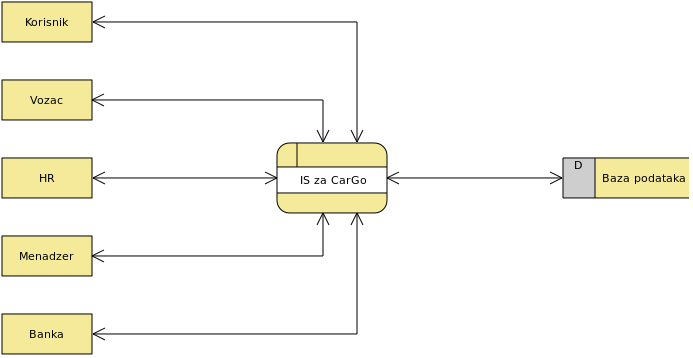
\includegraphics[width=\textwidth]{CarGoContextDiagram.png}
\end{center}
    \caption{Dijagram konteksta infomacionog sistema.}
\label{fig:CarGoContextDiagram}
\end{figure}

\begin{figure}[H]
\begin{center}
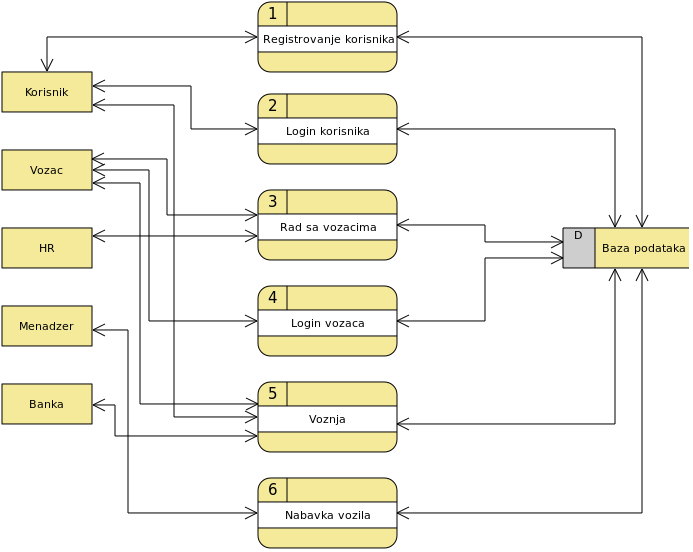
\includegraphics[width=\textwidth]{ISzaCarGo.png}
\end{center}
    \caption{Dijagram toka podataka nivoa 1.}
\label{fig:dtp1}
\end{figure}

\subsection{\bfseries Akteri}
\begin{itemize}
    \item Korisnici ovog sistema su svi oni kojima je potreban transport od jednog odredišta do drugog. Možemo ih podeliti na fizička i pravna lica. 
    \begin{itemize}
        \item Fizička lica - osobe koje usluge ovog sistema koriste preko svojih računa
        \item Pravna lica - osobe koje usluge ovog sistema koriste preko računa firme u kojoj rade
    \end{itemize}
    \item Vozači su ljudi kojima ovaj informacioni sistem posreduje kako bi izvršavali usluge korisnicima kojima je potreban prevoz. Vozači većinski koriste svoje automobile za prevoz.
    \item Banka je posrednik u transakciji između korisnika i vozača nakon izvršene usluge.
    \item Dobavljači vozila su grupa ljudi koja se bavi nabavkom dela vozila koja se koristi za prevoz korisnika
    \item HR tim je grupa ljudi koja odlučuje ko je podoban da bude vozač, odnosno ko je bezbedan po korisnike sistema i ima dozvolu za vozilo kojim upravlja. Ukoliko vozač nema svoje vozilo ovaj tim je dužan da o tome obavesti šefa voznog parka.
     \item Šef voznog parka je osoba koja je sastavlja porudžbine o broju vozila neophodnih vozačima koju šalje dobavljačima.
\end{itemize}
\section{\bfseries Slu\v cajevi upotrebe}

\subsection{\bfseries Registrovanje korisnika}
\subsection{\bfseries Login korisnika}
\subsection{\bfseries Rad sa voza\v cima}
\subsubsection{\bfseries Registrovanje voza\v ca}
\subsubsection{\bfseries Zahtev za automobil}
\subsubsection{\bfseries Otpu\v stanje voza\v ca}
\subsection{\bfseries Login voza\v ca}
\subsection{\bfseries Vo\v znja}
\subsubsection{\bfseries Naru\v civanje vo\v znje}
\subsubsection{\bfseries Prihvatanje vo\v znje}
\subsubsection{\bfseries Prevoz putnika}
\subsubsection{\bfseries Ocenjivanje voza\v ca}
\subsubsection{\bfseries Naplata vo\v znje}

\newpage

\subsubsection{\bfseries Kreiranje narudžbine vozila}
\noindent Slučaj upotrebe: Kreiranje narudžbine vozila:\\
1. Kratak opis:
\par -Šef voznog parka sastavlja porudžbinu o broju vozila pomoću informacije o vozačima kojima su potrebna vozila, a koju će kasnije proslediti dobavljaču vozila.\\
2. Učesnici:
\par -Šef voznog parka
\par -HR tim\\
3. Preduslovi:
\par -Postoje vozači kojima su potrebna vozila.\\
4. Postuslovi:
\par -Porudžbina je sastavljena i spremna da bude poslata.\\
5. Osnovni tok:
\par 1. HR tim šalje dopis šefu voznog parka na nedeljnom nivou koliko novih vozača nema svoje vozilo.
\par 2. Šef voznog parka proverava da li ima 10 ili više vozača kojima je potrebno vozilo ili postoji barem jedan vozač koji čeka na vozilo više od dve nedelje.
\par 3. Šef voznog parka sastavlja porudžbinu.\\

\noindent 6. Alternativni tok:
\par 2: Ima manje od 10 vozača kojima je potrebno vozilo ili nijedan vozač ne čeka 2 nedelje.
\par -Šef voznog parka čeka sledeći dopis od HR tima i kreće ponovo od koraka 2.

\subsubsection{\bfseries Nabavka vozila}
\noindent Slučaj upotrebe: Nabavka vozila\\
1. Kratak opis:
\par -Šef voznog parka ima zadatak da naruči potrebnu količinu vozila kako bi ih prosledio novozaposlenim vozačima koji nemaju svoja vozila.\\
2. Učesnici:
\par -Dobavljač
\par -Šef voznog parka\\
3. Preduslovi:
\par -Postoji barem jedan vozač koji nema svoje vozilo.\\
4. Postuslovi:
\par -Pribavljeno je onoliko vozila koliko ima vozača koji nemaju svoja.\\
5. Osnovni tok:
\par 1. Šef voznog parka proverava da li postoji neki vozač koji je zaposlen i čeka na firmu da mu pribavi vozilo.
\par 2. Šef voznog parka nakon provere sastavlja porudžbinu.
\par 3. Šef voznog parka stupa u kontakt sa dobavljačem.
\par 4. Šef voznog parka isporučuje dobavljaču zahtevan broj vozila.
\par 5. Dobavljač prihvata porudžbinu.
\par 6. Dobavljač isporučuje Šefu voznog parka zahtevan broj vozila.
\par 7. Šef voznog pa:rka ih smešta u vozni park do raspodele vozila vozačima.\\

\noindent 6. Alternativni tok:
	\par 5: U slučaju da dobavljač nije u stanu da ostvari porudžbinu
	\par	-Šef voznog parka odlaže nabavku u slučaju da su vozila potrebna za manje od 10 vozača.
	\par	-Šef voznog parka pronalazi drugog dobavljača u slučaju da postoji 10 ili više vozača koji čekaju na vozila i nastavlja do koraka 5.

\subsubsection{\bfseries Predaja vozila vozaču}
\noindent Slučaj upotrebe: Predaja vozila vozaču\\
1. Kratak opis: 
\par -Šef voznog parka prosleđuje vozilo iz voznog parka onom vozaču koji se zaposlio a nema svoje vozilo.\\
2. Učesnici:
\par -Šef voznog parka
\par -Vozač\\
3. Preduslovi:
\par -Vozač koji nema svoje vozilo pa čeka na firmino vozilo\\
4. Postuslovi:
\par -Vozaču je predato vozilo na korišćenje.\\
5. Osnovni tok:
\par 1. Šef voznog parka obaveštava vozača da li ima vozilo.
\par 2. Vozač i šef voznog parka se dogovaraju kada će se sastati.
\par 3. Vozač i šef voznog parka se nalaze.
\par 4. Vozač napismeno prihvata odgovornost za to vozilo.
\par 5. Vozač preuzima vozilo.\\

\noindent 6. Alternativni tok:
	\par 1: Šef voznog parka nema vozilo za vozača
	\par -Šef voznog parka dodaje vozača na spisak vozača koji čekaju na nabavku vozila nakon koje se kreće od koraka 1.
	
\subsubsection{\bfseries Upravljanje podacima o vozačima}

\subsubsection{\bfseries Upravljanje podacima o dobavljačima}
\newpage

\section{\bfseries Arhitektura sistema}

U ovom poglavlju biće prikazana predložena arhitektura sistema.

\subsection{\bfseries Karakteristike sistema}

Arhitektura sistema je razmatrana tako da odgovara sledećim ciljevima koje sistem treba da ispuni:
\begin{itemize}
    \item Bezbednost
    \item Stabilnost
    \item Jednostavnost upotrebe
    \item Dostupnost
    \item Odziv
\end{itemize}
Bezbednost i stabilnost su postignuti troslojnom arhitekturom dok je jednostavnost upotrebe je postignuta pažljivom izradom korisničkog interfejsa. Izborom mobilne aplikacije omogućava se postizanje visokog stepena dostupnosti, dok je dobar odziv je garantovan dokle god korisnik ima zadovoljavajuću internet konekciju.
Karakteristike arhitekture sistema za aplikaciju CarGo:
\begin{enumerate}
    \item Tip aplikacije: Mobilna aplikacija
    \item Strategije isporučivanja: Jedan serverski i više klijentskih računara
    \item Tehnologije: Android, Java, Geohash, Google S2 Geometry biblioteka
    \item Prateće komponente:
    \begin{enumerate}
        \item Logovanje na sistem: Podsistem za autentikaciju korisnika
        \item Praćenje vozila
        \item Lociranje korisnika
        \item Backup baze podataka: Podsistem koji automatski ili na zahtev pravi kopiju baze podataka
        \item Pomoć: Uputstvo za korišćenje veb aplikacije, kontakt forma, FAQ
    \end{enumerate}
\end{enumerate}

\newpage

\subsection{\bfseries Tip i slojevi arhitekture}

Za informacioni sistem je izabrana višeslojna klijent-server arhitektura koja se sastoji iz 3 sloja:
\begin{itemize}
    \item Prezentacioni sloj
    \item Logički sloj
    \begin{itemize}
        \item Klijentski kontroler
        \item Serverski kontroler
    \end{itemize}
    \item Sloj podataka
\end{itemize}

\subsubsection{\bfseries Prezentacioni sloj}

Predstavlja najviši sloj aplikacije i ima ulogu da korisniku
prikazuje i oslikava sadržaj koji dobija od nižih slojeva. Detaljniji prikaz je dat u sekciji Predlog izgleda korisničkog interfejsa. Ovaj sloj ima zadatak da korišćenje sistema učini efikasnijim i jednostavnijim i da korisnicima prikaže sve potrebne informacije koje dobije od nižih slojeva.
\newline
Sastoji se iz sledećih komponenti:
\begin{itemize}
    \item Registrovanje
    \item Prijavljivanje
    \item Naručivanje vožnje
    \item Ocenjivanje vozača
    \item Izmena ličnih podataka
\end{itemize}

\subsubsection{\bfseries Klijentski kontroler}

Glavni zadatak klijentskog kontrolera je da komunicira sa serverskim slojem sistema. Zadužen je da prosleđuje podatke prezentacionom sloju koji dalje korisnika obaveštava o ishodima njegovih akcija.
\newline
Sastoji se iz komponenti:
\begin{itemize}
    \item Validacija
    \item Dohvatanje podataka
    \item Autorizacija i autentifikacija
\end{itemize}

\subsubsection{\bfseries Serverski kontroler}

Serverski kontroler ima sličnu svrhu kao i klijentski kontroler, s tim što je obezbeđeno da klijenti nemaju pristup ovom delu aplikacije, prvenstveno zbog bezbednosti. Ovde se zbog toga vrše detaljnije autorizacije i validacije podataka kao i komunikacija sa bazom podataka. U ovom delu se takođe i izvršavaju neophodna izračunavanja nad podacima dobijenim iz baze.
\newline
Sastoji se iz komponenti:
\begin{itemize}
    \item Izačunavanje putanje vožnje
    \item Izračunavnje cene vožnje
    \item Naplaćivanje
    \item Autorizacija i autentifikacija
\end{itemize}
\subsubsection{\bfseries Sloj podataka}
Sadrži sve potrebne mehanizme za bezbedno pristupanje podacima u bazi podataka. Sloj podataka enkapsulira ove mehanizme i obezbeđuje lak pristup podacima. Zadatak mu je da dopusti pristup sloju iznad da koristi podatke na jednostavan način.

\begin{figure}[H]
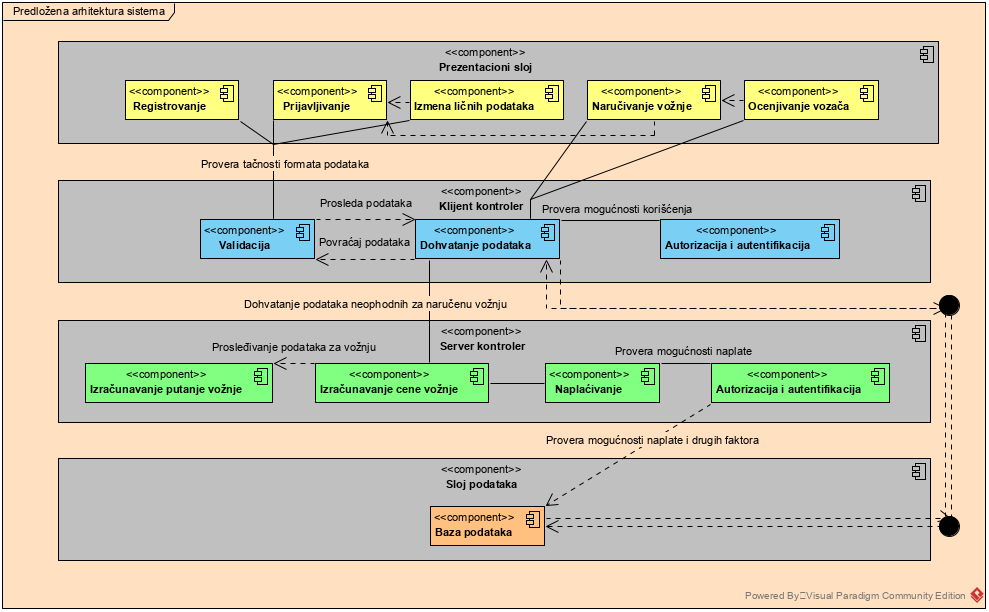
\includegraphics[scale = 0.70]{Slike/Arhitektura.png}
    \caption{Dijagram predložene arhitekture sistema.}
\label{fig:Predložena arhitektura sistema}
\end{figure}

\newpage

\section{\bfseries Opis baze podataka}
Baza podataka je projektovana tako da pokrije sve slučajeve upotrebe informacionog sistema aplikacije CarGo. Na slici \ref{fig:bazaPodataka} prikazana je šema baze.

\begin{figure}[H]
\begin{center}
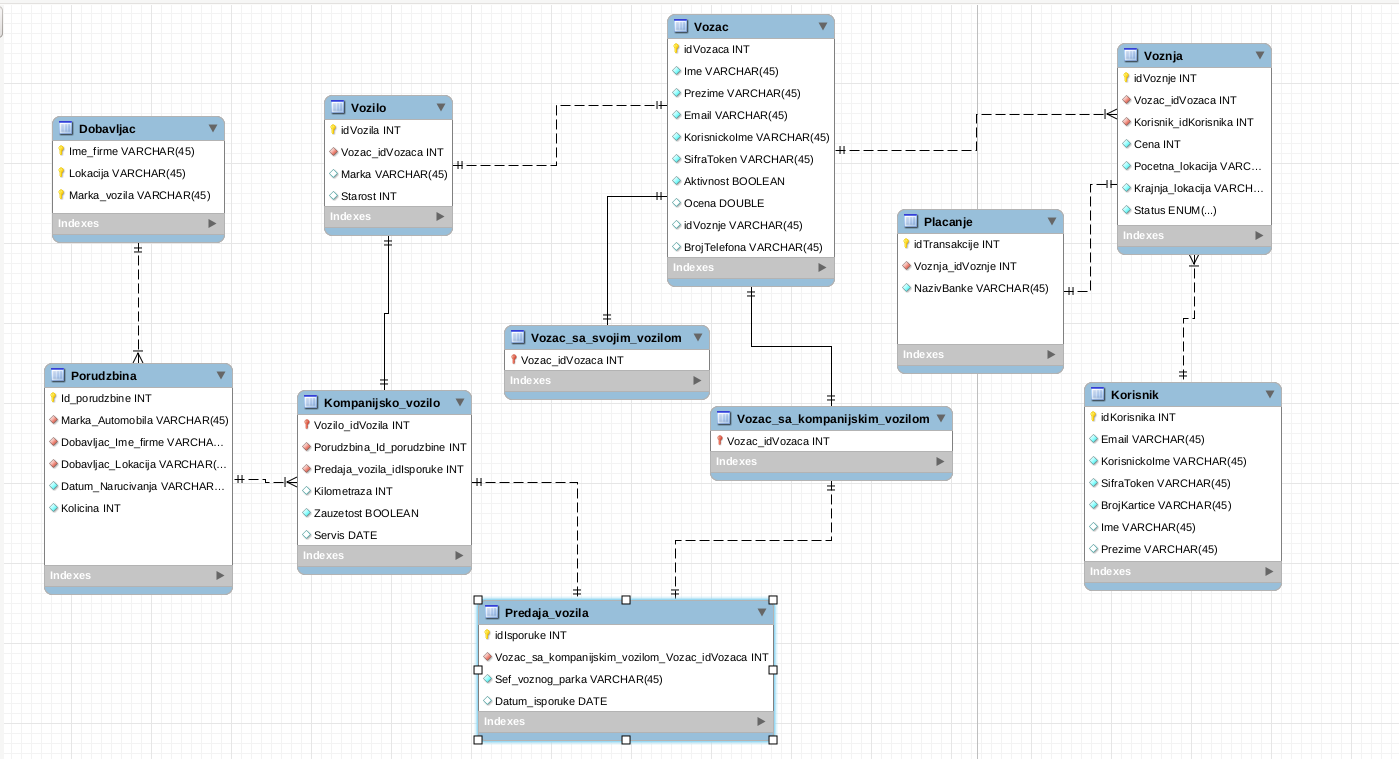
\includegraphics[width=\textwidth]{Slike/EERDijagramBazePodataka.png}
\end{center}
    \caption{Šema baze podataka}
\label{fig:bazaPodataka}
\end{figure}

\subsection{\textbf{Nezavisni entiteti}}Nezavisni entiteti su:
    \begin{itemize}
        \item Vozač
        \item Korisnik
        \item Vozilo
        \item Dobavljač
    \end{itemize}

\begin{flushleft}
\underline{Vozač}
\end{flushleft}
Svaki vozač ima email i šifru pomoću kojih pristupa svom nalogu. Vozač postaje aktivan kad se prijavi. Atributi:
\begin{itemize}
    \item Ime
    \item Prezime
    \item korisnickoIme - korisničko ime vozača pomoću kojeg se prijavljuje
    \item Ocena - ocena koju je dobio od korisnika u određenoj vožnji
    \item Email - email sa kojim se vozač registrovao
    \item SifraToken - enkriptovana sifra vozača
    \item Aktivnost - trenutno stanje vozača, može biti aktivan ili neaktivan
    \item IdVoznje - vožnje u kojima je vozač učestvovao
    \item BrojTelefona
\end{itemize}

\begin{flushleft}
\underline{Korisnik}
\end{flushleft}
Kao i vozač, i korisnik ima svoj nalog. Korisnik se prijavljuje kad mu je potrebna vožnja. Za registraciju mora koristiti email. Atributi:
\begin{itemize}
    \item Ime
    \item Prezime
    \item KorisnickoIme - korisničko ime pomoću kojeg se korisnik prijavljuje
    \item Email - email korisnika pomoću kojeg se registruje
    \item SifraToken - enkriptovana šifra korisnika
    \item BrojKartice - broj kartice pomoću koje korisnik vrši plaćanje
\end{itemize}

\begin{flushleft}
\underline{Vozilo}
\end{flushleft}
Sadrži informacije o vozilima svih vozača. Atributi:
\begin{itemize}
    \item Vozac\_idVozaca - Id vozača koji koristi to vozilo
    \item Marka
    \item Starost
\end{itemize}

\begin{flushleft}
\underline{Dobavljač}
\end{flushleft}
Sadrži informacije o dobavljačima od kojih nabavljamo vozila. Atributi:
\begin{itemize}
    \item Ime\_firme
    \item Lokacija
    \item Marka\_vozila
\end{itemize}


\subsection{\textbf{Izvedeni entiteti}}
Izvedeni entiteti su:
\begin{itemize}
    \item Vozač sa svojim vozilom
    \item Vozač sa kompanijskim vozilom
    \item Kompanijsko vozilo
\end{itemize}

\begin{flushleft}
\underline{Vozač sa svojim vozilom}
\end{flushleft}
Predstavlja specijalizaciju eniteta vozač. Sadrži informacije o vozačima koji imaju sopstveno vozilo. Atributi:
\begin{itemize}
    \item Vozac\_idVozaca - Id vozača koji ima sopstveno vozilo, strani ključ ka entitetu vozač
\end{itemize}

\begin{flushleft}
\underline{Vozač sa kompanijskim vozilom}
\end{flushleft}
Predstavlja specijalizaciju entiteta vozač. Sadrži informacije o vozačima koji nemaju sopstveno vozilo. Atributi:
\begin{itemize}
    \item Vozac\_idVozaca - Id vozača koji nema sopstveno vozilo, strani ključ ka entitetu vozač
\end{itemize}

\begin{flushleft}
\underline{Kompanijsko vozilo}
\end{flushleft}
Predstavlja specijalizaciju entiteta vozilo. Sadrži informacije o vozilima koji su u vlasnistvu firme i izdaju se vozačima na korišćenje. Atributi:
\begin{itemize}
    \item Vozilo\_idVozila - strani ključ ka entitetu vozilo.
    \item Porudzbina\_id\_porudzbine - redni broj porudžbine u kojoj je vozilo naručenoču.
    \item Predaja\_vozila\_idisporuke - strani ključ na tabelu predaja vozila
    \item Zauzetost - indikator da li je vozilo predato nekom vozaču ili ne
    \item Kilometraza
    \item Servis
\end{itemize}


\subsection{\textbf{Agregirani entiteti}}
Agregirani entiteti su:
\begin{itemize}
    \item Vožnja
    \item Plaćanje
    \item Predaja vozila
    \item Porudžbina
\end{itemize}

\begin{flushleft}
\underline{Vožnja}
\end{flushleft}
Sadrži informacije o svim vožnjama. Atributi:
\begin{itemize}
    \item Vozac\_idVozaca - id vozača koji vozi korisnika ka željenoj lokaciji, strani ključ ka entitetu Vozač.
    \item Vozac\_idKorisnika - id korisnika koji je traži prevoz, strani ključ ka entitetu Korisnik.
    \item Cena - naknada koju korisnik treba da plati za izvršenu uslugu.
    \item Pocetna\_lokacija - lokacija sa koje je korisnik zatrašio uslugu.
    \item Krajnja\_lokacija - lokacija na koju korisnik želi da se preveze.
    \item Status - trenutni status vožnje.
\end{itemize}

\begin{flushleft}
\underline{Plaćanje}
\end{flushleft}
Sadrži informacije o platnim transakcijama za svaku vožnju. Atributi:
\begin{itemize}
    \item Voznja\_idVoznje - id vožnje za koju se vrši plaćanje.
    \item NazivBanke - Naziv banke koja vrši transakciju.
\end{itemize}

\begin{flushleft}
\underline{Predaja vozila}
\end{flushleft}
Sadrži informacije o predatim vozilima vozačima koji nemaju svoja. Atributi:
\begin{itemize}
    \item Vozac\_sa\_kompanijskim\_vozilom\_Vozac\_idVozaca - strani ključ na entitet Vozač sa kompanijskim vozilom.
    \item Sef\_voznog\_parka - ime osobe koja vrši dobavljanje vozila.
    \item Datum
\end{itemize}

\begin{flushleft}
\underline{Porudžbina}
\end{flushleft}
Sadrži informacije o naručenim vozilima vozačima koji nemaju svoja. Atributi:
\begin{itemize}
    \item Marka\_automobila - strani ključ na entitet Dobavljač, sadrži informacije o marki automobila koji se naručuje.
    \item Dobavljac\_ime\_firme - strani ključ na entitet Dobavljač, sadrži informacije o nazivu firme od koje naručujemo vozila.
    \item Dobavljac\_Lokacija - strani ključ na entitet Dobavljač, sadrži informacije o lokaciji firme od koje naručujemo vozila.
    \item Datum\_narucivanja
    \item Kolicina - broj vozila koji se naručuje.
\end{itemize}

\section{\bfseries Predlog korisničkog interfejsa}

U ovom poglavlju će biti prikazan zamišljen izgled korisničkog interfejsa ove aplikacije. Aplikaciju koriste zaposleni kao i korisnici. U narednim podsekcijama biće prikazane slike određenih delova aplikacije uz kratko objašnjenje.

\subsection{\bfseries Registrovanje korisnika}

Način registrovanja korisnika je prikazan na slici \ref{fig:Registrovanje korisnika}. Registrovanje se sastoji od unošenja korisničkog imena, mejla i lozinke.  Izvršava se klikom na dugme \say{Sign Up}. Registrovani korisnik može klikom na dugme \say{Sign in} da se prijavi kao što je objašnjeno u sekciji \ref{Prijavljivanje_korisnika_sekcija}.

\begin{figure}[H]
\begin{center}
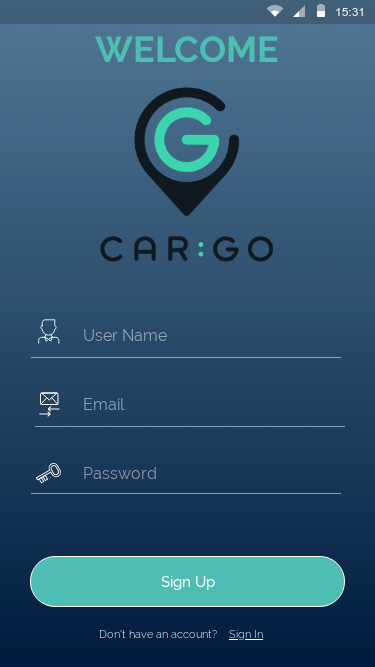
\includegraphics[width=4cm]{Slike/Registrovanje.png}
\end{center}
    \caption{Registrovanje korisnika}
\label{fig:Registrovanje korisnika}
\end{figure}

\subsection{\bfseries Prijavljivanje korisnika}
\label{Prijavljivanje_korisnika_sekcija}

Prijavljivanje korisnika (slika \ref{fig:Prijavljivanje korisnika}) koristi postojeće korisničko ime i lozinku. Prijavljivanje se izvršava klikom na dugme \say{Sign In} nakon ispravno unešenog korisničkog imena i lozinke.
\begin{figure}[H]
\begin{center}
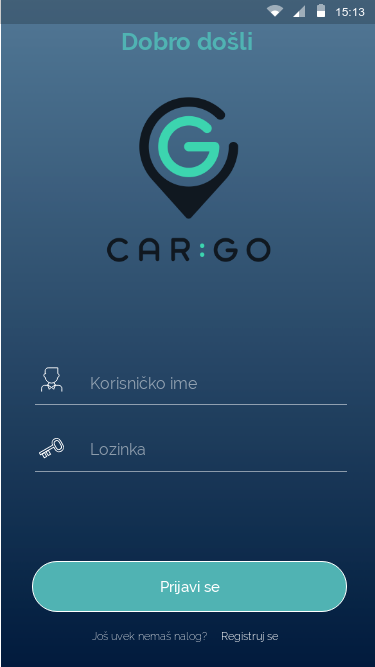
\includegraphics[width=4cm]{Slike/Prijavljivanje.png}
\end{center}
    \caption{Prijavljivanje korisnika}
\label{fig:Prijavljivanje korisnika}
\end{figure}


\subsection{\bfseries Profil korisnika}

Nakon uspešnog prijavljivanja na svoj nalog, korisniku se prikazuje prva strana (slika \ref{fig:Profil korisnika}) na kojoj korisnik može da naruči vožnju, podesi informacije o kreditnoj kartici i da se odjavi. Klikom na dugme \say{Podešavanja kreditne kartice} korisniku se otvara nov prozor (slika \ref{fig:Podešavanje kartice}) u koji treba uneti sve potrebne informacije o kartici kako bi plaćanje moglo da bude realizovano. Ukoliko se klikne na dugme \say{Naručivanje vožnje} otvara se novi prozor u kome korisnik može da naruči vožnju (videti sekciju \ref{Naručivanje vožnje}).


\begin{figure}[h!]
\centering
\begin{minipage}{.5\textwidth}
  \centering
  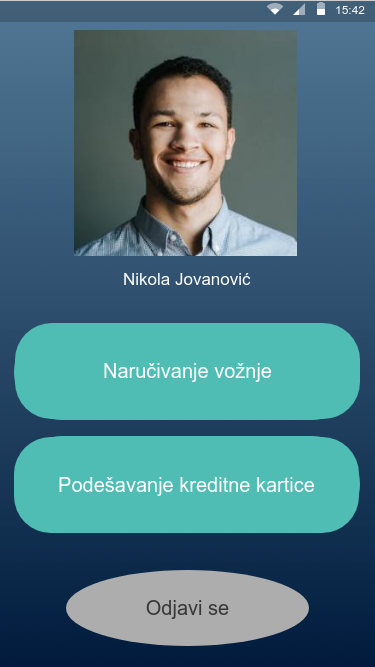
\includegraphics[width=.4\linewidth]{Slike/Profil.png}
  \caption{Profil korisnika}
  \label{fig:Profil korisnika}
\end{minipage}%
\begin{minipage}{.5\textwidth}
  \centering
  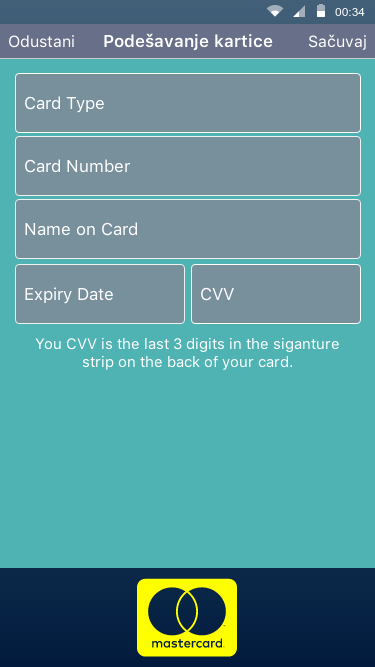
\includegraphics[width=.4\linewidth]{Slike/upravljanje_karticom.png}
   \caption{Podešavanje kartice}{}
  \label{fig:Podešavanje kartice}
\end{minipage}
\end{figure}


\subsection{\bfseries Naručivanje vožnje}
\label{Naručivanje vožnje}

Za naručivanje vožnje, korisniku je omogućeno da unese željenu lokaciju (slika \ref{fig:Naručivanje vožnje}). Nakon toga, aplikacija mu omogućava da vidi cenu vožnje klikom na dugme \say{Procenjena cena} (slika \ref{fig:Procena cene}).


\begin{figure}[H]
\centering
\begin{minipage}{.5\textwidth}
  \centering
  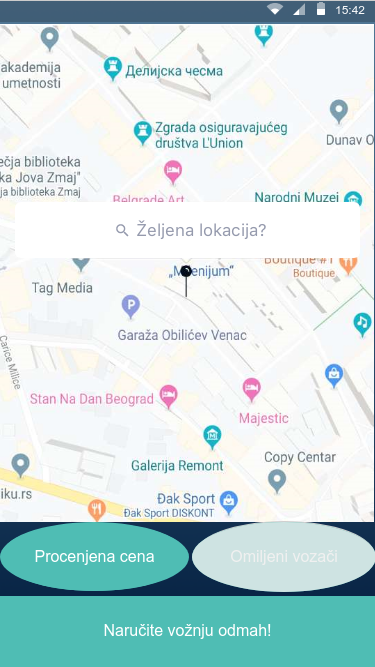
\includegraphics[width=.4\linewidth]{Slike/Narucivanje_sa_adresom.png}
  \caption{Naručivanje vožnje}{}
  \label{fig:Naručivanje vožnje}
\end{minipage}%
\begin{minipage}{.5\textwidth}
  \centering
  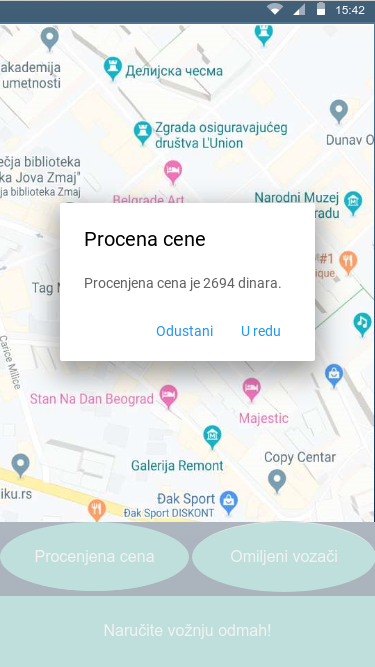
\includegraphics[width=.4\linewidth]{Slike/Procena_cene.png}
   \caption{Procena cene}{}
  \label{fig:Procena cene}
\end{minipage}
\end{figure}

Kada korisnik klikne na \say{Naručite vožnju odmah} vrši se pretraga slobodnih vozača najbiližih trenutnoj lokaciji korisnika (slika \ref{fig:Pronalazenje vozaca}). U ovoj fazi korisnik može prekinuti pretragu klikom na \say{Odustani} ukoliko se predomisli i više ne želi vožnju.

\begin{figure}[H]
\begin{center}
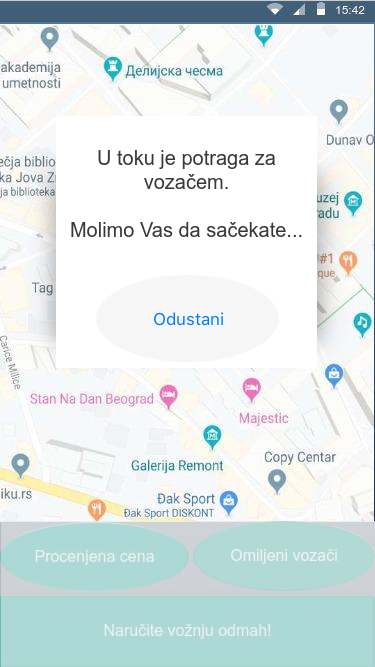
\includegraphics[width=4cm]{Slike/Pronalazenje_vozaca.png}
\end{center}
    \caption{Pronalaženje vozača}
\label{fig:Pronalazenje vozaca}
\end{figure}


Kada se završi pretraga korisnik dobija listu svih pogodnih vozača i bira onog kog želi (slike \ref{fig:Vozaci na raspolaganju} i \ref{fig:Prihvacena voznja}).

\begin{figure}[H]
\centering
\begin{minipage}{.5\textwidth}
  \centering
  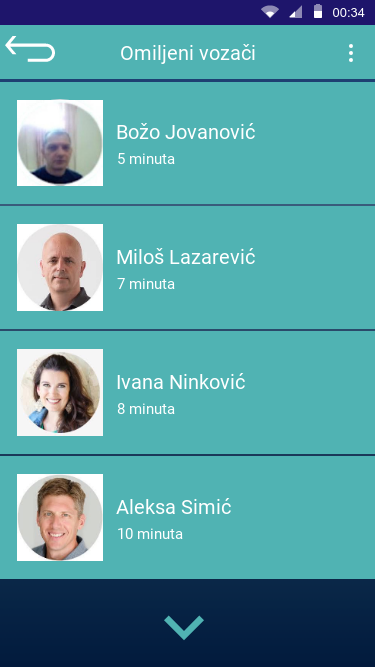
\includegraphics[width=.4\linewidth]{Slike/vozaci_na_raspolaganju.png}
  \caption{Vozači na raspolaganju}
  \label{fig:Vozaci na raspolaganju}
\end{minipage}%
\begin{minipage}{.5\textwidth}
  \centering
  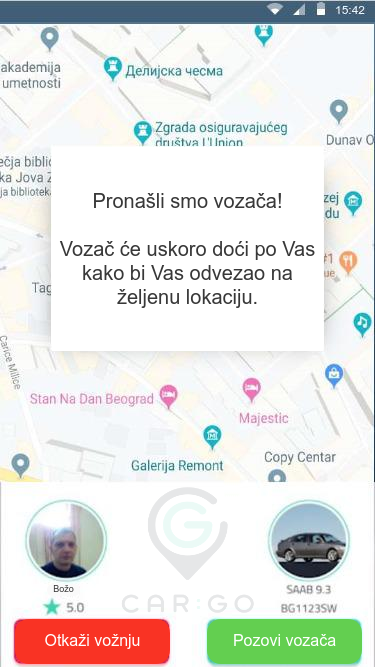
\includegraphics[width=.4\linewidth]{Slike/Prihvacena_voznja.png}
   \caption{Prihvaćena vožnja}
   \label{fig:Prihvacena voznja}
\end{minipage}
\end{figure}

\newpage

\subsection{\bfseries Završetak vožnje}

Nakon završene vožnje sistem nudi korisniku mogućnost da oceni i napiše neki komentar o vozaču ukoliko to želi (slika \ref{fig:Ocenjivanje vozaca}).

\begin{figure}[h!]
\begin{center}
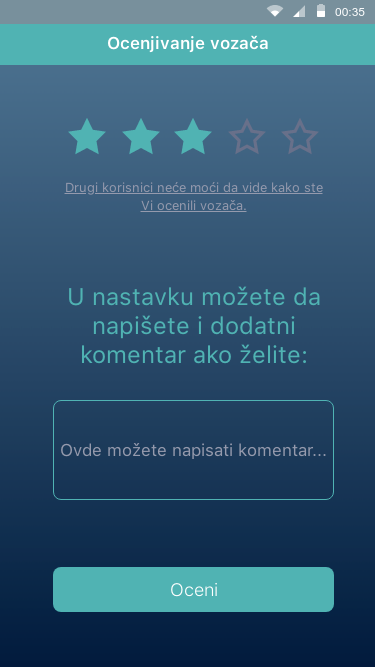
\includegraphics[width=4cm]{Slike/ocenjivanje_vozaca.png}
\end{center}
    \caption{Ocenjivanje vozača}
\label{fig:Ocenjivanje vozaca}
\end{figure}














\newpage

\end{document}
